\documentclass{article}
\usepackage[utf8]{inputenc}

\title{Assignment-3\\Fork assignment-2}
\author{Subash Mylraj \\(CED18I051) }
\date{16 September 2020}

\usepackage{geometry}
 \geometry{
 a4paper,
 total={170mm,257mm},
 left=20mm,
 top=10mm,
 }

\usepackage{longtable}
\usepackage{graphicx}
\usepackage{listings}
\usepackage{xcolor}

\begin{document}

\maketitle

\lstset{
  language=c,
  aboveskip=3mm,
  belowskip=3mm,
  showstringspaces=false,
  columns=flexible,
  basicstyle={\small\ttfamily},
  numbers=none,
  numberstyle=\tiny\color{gray},
  keywordstyle=\color{blue},
  commentstyle=\color{dkgreen},
  stringstyle=\color{mauve},
  breaklines=true,
  breakatwhitespace=true,
  tabsize=3
}

\definecolor{dkgreen}{rgb}{0,0.6,0}
\definecolor{gray}{rgb}{0.5,0.5,0.5}
\definecolor{mauve}{rgb}{0.58,0,0.82}

\section*{Question 1: Test Drive all the examples discussed so far in the class for the usage of wait, exec call variants.}

\bigskip

\textbf{\LARGE Code 1:}
\smallskip
\par\noindent\rule{\textwidth}{0.4pt}
\lstinputlisting[language=c]{src/1_1.c}
\par\noindent\rule{\textwidth}{0.4pt}

\bigskip
\noindent
\textbf{\LARGE Output:}

\begin{figure}[ht]
    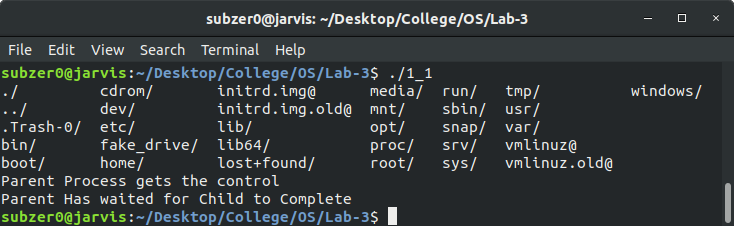
\includegraphics[width=\textwidth]{output/1_1.png}
\end{figure}
\bigskip
\bigskip
\bigskip

\bigskip

\noindent
\textbf{\LARGE Code 2:}
\smallskip
\par\noindent\rule{\textwidth}{0.4pt}
\lstinputlisting[language=c]{src/1_2.c}
\par\noindent\rule{\textwidth}{0.4pt}

\bigskip
\noindent
\textbf{\LARGE Output:}

\begin{figure}[ht]
    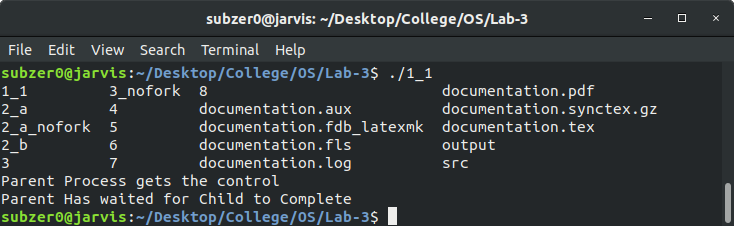
\includegraphics[width=\textwidth]{output/1_2.png}
\end{figure}
\bigskip
\bigskip
\bigskip

\noindent
\textbf{\LARGE Code 3:}
\smallskip
\par\noindent\rule{\textwidth}{0.4pt}
\lstinputlisting[language=c]{src/1_3.c}
\par\noindent\rule{\textwidth}{0.4pt}

\bigskip
\noindent
\textbf{\LARGE Output:}

\begin{figure}[ht]
    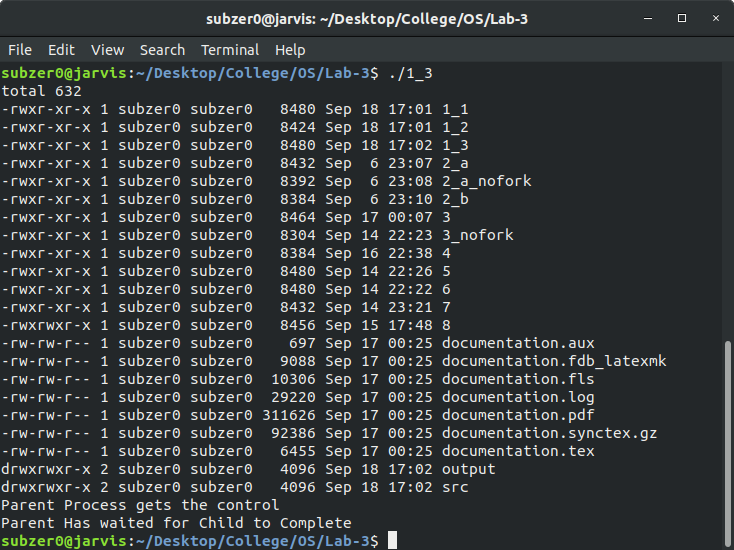
\includegraphics[width=\textwidth]{output/1_3.png}
\end{figure}
\bigskip
\bigskip
\bigskip

\noindent
\textbf{\LARGE Code 4:}
\smallskip
\par\noindent\rule{\textwidth}{0.4pt}
\lstinputlisting[language=c]{src/1_4.c}
\par\noindent\rule{\textwidth}{0.4pt}

\bigskip
\noindent
\textbf{\LARGE Output:}
\\
\begin{figure}[h]
    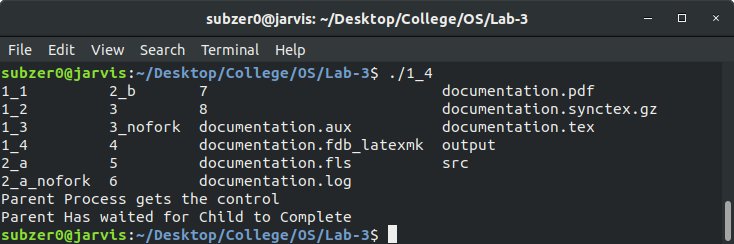
\includegraphics[width=\textwidth]{output/1_4.png}
\end{figure}

\bigskip
\bigskip
\bigskip

\pagebreak
\section*{Question 2.a: Odd and Even series generation for n terms using Parent Child relationship (say odd is the duty of the parent and even series as that of child)}

\begin{longtable}{c c}
    % \centering
    \begin{tabular}{c|c }
        \hline
        Forked Implementation & Non Forked implementation \\
        \hline
        \lstinputlisting[language=c]{src/2_a.c} & \lstinputlisting[language=c]{src/2_a_nofork.c} \\
        \hline
        \multicolumn{2}{c}{Running and timing both the programs for input of 100000 is as follows:} \\
        \hline
        0m0.73s & 0m0.109s \\
        \hline
        \multicolumn{2}{c}{Output: for input n=10} \\
        \hline
        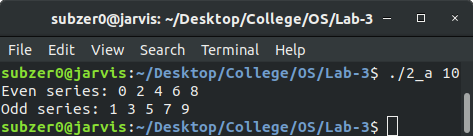
\includegraphics[width=3in]{output/2.png}
        &
        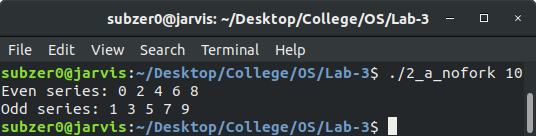
\includegraphics[width=3.33in]{output/2_nofork.png}

    \end{tabular}
    % \caption{Caption}
    \label{tab:my_label}
\end{longtable}

\section*{Question 2.b: given a series of n numbers ( u can assume natural numbers till n) generate the sum of odd terms in the parent and the sum of even terms in the child process}

\bigskip

\textbf{\LARGE Code:}
\smallskip
\par\noindent\rule{\textwidth}{0.4pt}
\lstinputlisting[language=c]{src/2_b.c}
\par\noindent\rule{\textwidth}{0.4pt}

\bigskip
\noindent
\textbf{\LARGE Output:}

\begin{figure}[ht]
    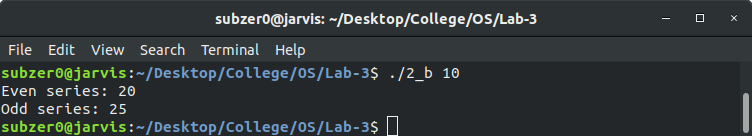
\includegraphics[width=\textwidth]{output/2_b.png}
\end{figure}
\bigskip
\bigskip
\bigskip

\section*{Question 3: Armstrong number generation within a range. The digit extraction, cubing can be responsibility of child while the checking for sum == no can happen in child and the output list in the child.}

\bigskip

\textbf{\LARGE Code:}
\smallskip
\par\noindent\rule{\textwidth}{0.4pt}
\lstinputlisting[language=c]{src/3.c}
\par\noindent\rule{\textwidth}{0.4pt}

\bigskip
\noindent
\textbf{\LARGE Output:}
\bigskip \\Something to be noted here is that, this question is not asking for a 
efficient parallelized output. Since this assignment is to train one's 
skills in using fork, this code does not efficiently parallelize output.
Nevertheless, the required output using the algorithm stated in the question
is as follows.\\
\begin{figure}[ht]
    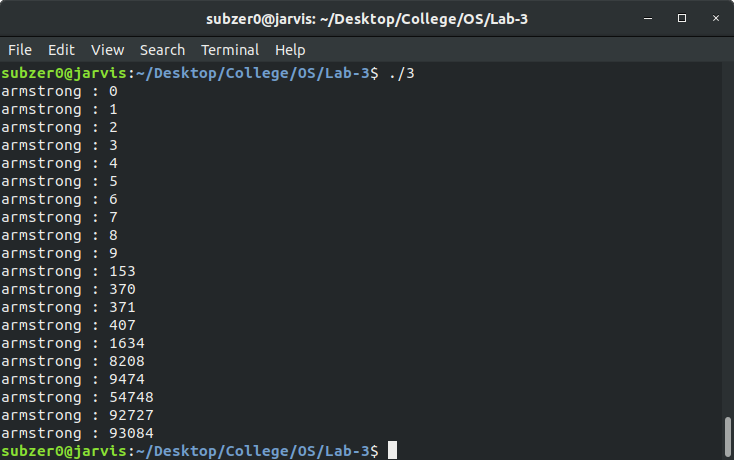
\includegraphics[width=\textwidth]{output/3.png}
\end{figure}


\section*{Question 4: Fibonacci Series AND Prime parent child relationship (say parent does fib Number generation using series and child does prime series)}

\bigskip

\textbf{\LARGE Code:}
\smallskip
\par\noindent\rule{\textwidth}{0.4pt}
\lstinputlisting[language=c]{src/4.c}
\par\noindent\rule{\textwidth}{0.4pt}

\bigskip
\noindent
\textbf{\LARGE Output:}
\bigskip \\This code generates a series of length n for both Fibonacci
and prime series. Both the series are generated in parallel. The child
process takes care of generating the prime series while the parent process
process takes care of generating the Fibonacci series.

\begin{figure}[ht]  
  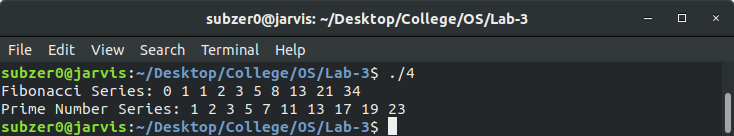
\includegraphics[width=\textwidth]{output/4.png}
\end{figure}


\section*{Question 5: Ascending Order sort within Parent and Descending order sort (or vice versa) within the child process of an input array. (u can view as two different outputs –first entire array is asc order sorted in op and then the second part desc order output)}

\bigskip

\textbf{\LARGE Code:}
\smallskip
\par\noindent\rule{\textwidth}{0.4pt}
\lstinputlisting[language=c]{src/5.c}
\par\noindent\rule{\textwidth}{0.4pt}

\bigskip
\noindent
\textbf{\LARGE Output:}
\bigskip \\This code sorts the given array in both ascending and descending
order. Both the sorts are done in parallel. The child process takes care of 
sorting the array in ascending order while the parent process takes care of
sorting the array in descending order.
\begin{figure}[ht]
    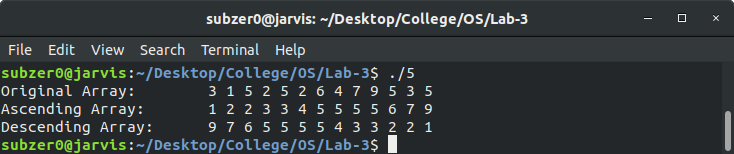
\includegraphics[width=\textwidth]{output/5.png}
\end{figure}

\section*{Question 6: Given an input array use parent child relationship to sort the first half of array in ascending order and the trailing half in descending order (parent / child is ur choice)}

\bigskip

\textbf{\LARGE Code:}
\smallskip
\par\noindent\rule{\textwidth}{0.4pt}
\lstinputlisting[language=c]{src/6.c}
\par\noindent\rule{\textwidth}{0.4pt}

\bigskip
\noindent
\textbf{\LARGE Output:}
\bigskip \\This code sorts the first half of the array in ascending and the
other half in descending order. vfork() was used to achieve this goal. One
thing to be noted is that, vfork does not achieve true parallelism when used.
So this code is not a parallelized implementation but rather a multiprocessed
implementation.
\begin{figure}[ht]
    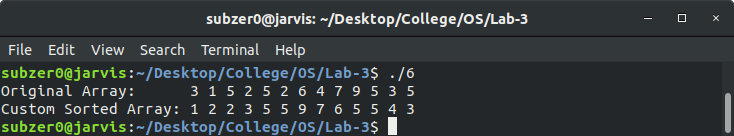
\includegraphics[width=\textwidth]{output/6.png}
\end{figure}

\section*{Question 7: Implement a multiprocessing version of binary search where the parent searches for the key in the first half and subsequent splits while the child searches in the other half of the array. By default u can implement a search for the first occurrence and later extend to support multiple occurrence (duplicated elements search as well)}

\bigskip

\textbf{\LARGE Code:}
\smallskip
\par\noindent\rule{\textwidth}{0.4pt}
\lstinputlisting[language=c]{src/7.c}
\par\noindent\rule{\textwidth}{0.4pt}

\bigskip
\noindent
\textbf{\LARGE Output:}
\bigskip \\This code implements a search algorithm (non-sorted array) by initially checking if the
middle element is the key. If not, then both the left and the right sub-halves are checked in the same
recursively. The checking for the left and right sub-halves is done using forks. Hence this is a parallelized
implementation. This is slightly similar to that of binary search in the fact that the middle element
is checked in every iteration.

\begin{figure}[ht]
    The inputs can be viewed at the program source code.\\ 
    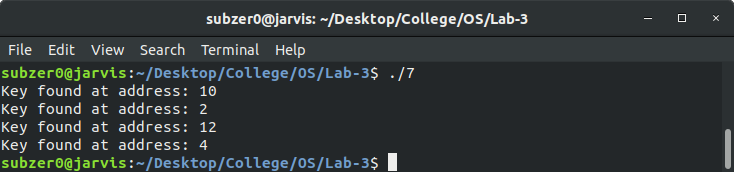
\includegraphics[width=\textwidth]{output/7.png}
\end{figure}

\section*{Question 8: * Non Mandatory [extra credits] Read upon efficient ways of parallelizing the generation of Fibonacci series and apply the logic in a parent child relationship to contributes a faster version of fib series generation as opposed to sequential logic in (4)}

\bigskip

\textbf{\LARGE Code:}
\smallskip
\par\noindent\rule{\textwidth}{0.4pt}
\lstinputlisting[language=c]{src/8.c}
\par\noindent\rule{\textwidth}{0.4pt}

\bigskip
\noindent
\textbf{\LARGE Output:} \\
    One thing to note here is that Fibonacci series depends on its previous
    2 elements. Hence whatever algo is used, to calculate the nth element, 
    its previous elements have to be calculated. So, the time complexity 
    can never be below O(n). \\
    For example, to calculate fib(7), we need to find fib(6), fib(5), ... 
    fib(2), fib(1). To calculate fib(6), we need to find fib(5), fib(4), ... 
    fib(2), fib(1). Hence finding all these in a linear sequential manner would
    lead to a time complexity of about O($2^n$). \\
    But with parallelization or by calculating the series till n from a bottom up
    manner, we can get the time complexity down to O(n).
\begin{figure}[ht]
    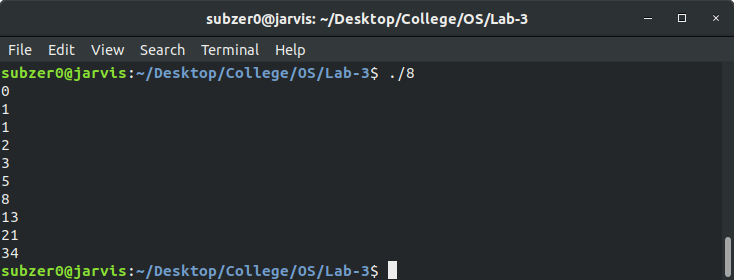
\includegraphics[width=\textwidth]{output/8.png}
\end{figure}

\end{document}